\chapter*{About the Author}
\addcontentsline{toc}{chapter}{About the Author}
\markboth{About the Author}{About the Author}

\noindent

\begin{minipage}[t]{0.60\textwidth}

    \small

    \setlength{\parskip}{0.45em}
    \setlength{\parindent}{0pt}

    \textbf{\BookletAuthor} (\BookletAuthorHandle) is a Computer
    Engineering student and open-source developer with a lifelong pull
    toward computers, going back to around age four, when they were
    mostly a source of curiosity and games. At thirteen or fourteen,
    long before he wrote any code, he wrote his first book: a short,
    fictional story about dinosaurs.

    That same curiosity later turned into backend engineering and a
    string of open-source developer tools. Writing about data structures
    and algorithms eventually ran into a wall: sections he could produce
    mechanically but not really explain. \textit{Mathesis} is what
    started when he went back to fix that --- to the logic, sets, and
    proofs everything else quietly assumes --- and this booklet is one
    piece of that ongoing return to first principles.

\end{minipage}%
\hspace{0.025\textwidth}%
\begin{minipage}[t]{0.34\textwidth}

    \centering

    \vspace{0pt}

    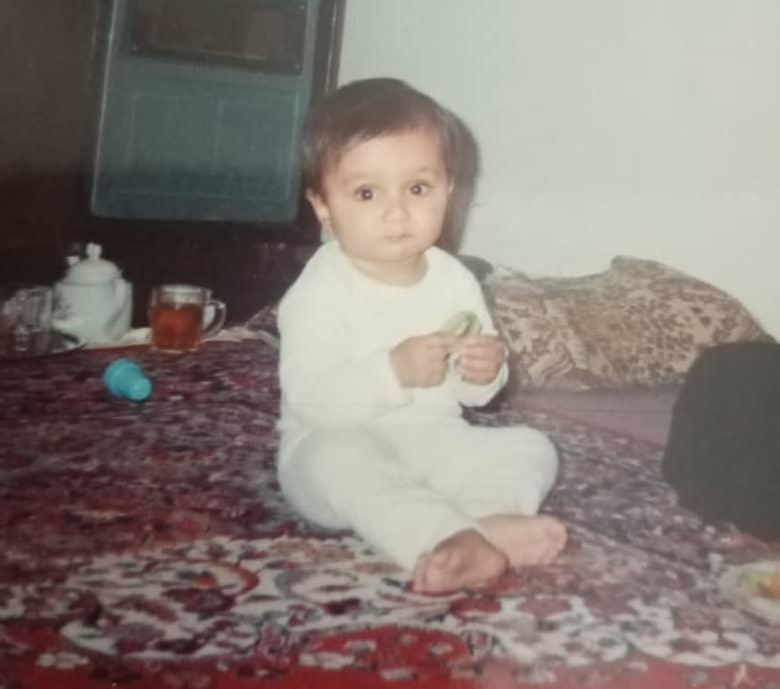
\includegraphics[width=\linewidth]{../../shared/images/author-photo.jpg}

\end{minipage}

\medskip

\noindent

\begin{tabular}{@{}ll}
Email:      & \href{mailto:\BookletEmail}{\BookletEmail} \\
Handle:     & \BookletAuthorHandle \\
Repository: & \href{https://github.com/papyrxis/mathesis}
              {github.com/papyrxis/mathesis} \\
\end{tabular}

\clearpage
